%\documentclass[landscape,a0b,final,a4resizeable]{a0poster}
%\documentclass[landscape,a0b,final]{a0poster}
%\documentclass[portrait,a0b,final,a4resizeable]{a0poster}
\documentclass[portrait,a0,final]{a0poster} %changed document class from a0b to a0 otherwise the second column extends out side the page

%%% Option "a4resizeable" makes it possible ot resize the
%   poster by the command: psresize -pa4 poster.ps poster-a4.ps
%   For final printing, please remove option "a4resizeable" !!

\usepackage{epsfig}
\usepackage{multicol}
\usepackage{pstricks,pst-grad}




%%%%%%%%%%%%%%%%%%%%%%%%%%%%%%%%%%%%%%%%%%%
% Definition of some variables and colors
%\renewcommand{\rho}{\varrho}
%\renewcommand{\phi}{\varphi}
\newrgbcolor{nus_blue}{0 0.129 0.388}
\newrgbcolor{nus_gold}{1 0.259 0}
\newrgbcolor{nus_lite}{1 0.259 0}
\newrgbcolor{lite}{.70 .70 .70}
\newrgbcolor{liter}{.95 .95 .95}
\setlength{\columnsep}{3cm}
% \setlength{\columnseprule}{2mm}
\setlength{\parindent}{0.0cm}


%% Figures and tables
%% The multicols package doesn't support the floats, figure and table.
%% Use tablehere and figurehere in place of table and figure.

\makeatletter
\newenvironment{tablehere}
  {\def\@captype{table}}
  {}

\newenvironment{figurehere}
  {\def\@captype{figure}}
  {}
\makeatother


% \figcaption replaces - replacement for \caption
% necessary, since in the multicols environment \figure and
% therefore \caption won't work

\newcommand{\ket}[1]{|{#1}\rangle}
\newcommand{\bra}[1]{\langle{#1}|}
\newcommand{\braket}[1]{\langle{#1}\rangle}

\setcounter{figure}{1}
\newcommand{\figcaption}[1]{
  \vspace{0.5cm}
  \begin{center}
  \begin{quote}
    {\large {\sc Figure} \arabic{figure}: #1}
  \end{quote}
  \end{center}
 % \vspace{1cm}
  \stepcounter{figure}
}

\setcounter{table}{1}
\newcommand{\tabcaption}[1]{
  \vspace{0.5cm}
  \begin{center}
  \begin{quote}
    {\normalsize {\sc Table} \arabic{table}: #1}
  \end{quote}
  \end{center}
 % \vspace{1cm}
  \stepcounter{table}
}
%%%%%%%%%%%%%%%%%%%%%%%%%%%%%%%%%%%%%%%%%%%%%%%%%%%%
%%%                Poster                        %%%
%%%%%%%%%%%%%%%%%%%%%%%%%%%%%%%%%%%%%%%%%%%%%%%%%%%%

\newenvironment{poster}{
  \begin{center}
  \begin{minipage}[c]{0.98\textwidth}
}{
  \end{minipage} 
  \end{center}
}




%%%%%%%%%%%%%%%%%%%%%%%%%%%%%%%%%%%%%%%%%%%%%%%%%%%%%%%%%%%%%%%%%%%%%%
%%% Begin of Document
%%%%%%%%%%%%%%%%%%%%%%%%%%%%%%%%%%%%%%%%%%%%%%%%%%%%%%%%%%%%%%%%%%%%%%

\begin{document}

\newrgbcolor{lightblue}{0. 0. 0.80}
\newrgbcolor{white}{1. 1. 1.}
\newrgbcolor{whiteblue}{.80 .80 1.}

\begin{poster}
\large \sf
\vspace{2cm}
%%%%%%%%%%%%%%%%%%%%%
%%% Header
%%%%%%%%%%%%%%%%%%%%%
\begin{center}

      %%% CQT_Logo
      \begin{minipage}[c]{0.05\textwidth}
        \begin{center}
          \includegraphics[width=14cm,angle=0]{CQT_Logo_CMYK.jpg}
        \end{center}
      \end{minipage}\hspace{10cm}
      %%% Title
      \begin{minipage}[c]{0.7\textwidth}
        \begin{center}
          {\sc \huge Cavity Quantum Electrodynamics With  \\ \vspace{0.8cm}
          
A Nearly Concentric Optical Cavity}\\[9mm]
          {\large Chi Huan Nguyen, Adrian Nugraha Utama, Nick Lewty, Christian Kurtsiefer}\\[6mm]
          Centre for Quantum Technologies, National University of Singapore, Singapore\\
          
        \end{center}
      \end{minipage}
      %%% NUS-Logo
      \begin{minipage}[l]{0.1\textwidth}
        \begin{center}
          \includegraphics[width=8cm,angle=0]{NUS_logo_full-horizontal.jpg}
        \end{center}
      \end{minipage}
\end{center}

\vspace{0.2cm}



%%%%%%%%%%%%%%%%%%%%%
%%% Content
%%%%%%%%%%%%%%%%%%%%%
\vspace{1cm}
\begin{multicols}{2}
\setlength{\parskip}{1ex plus 0.5ex minus 0.2ex}

      \begin{center}
          \begin{center}{\bf \Large \textsf {Motivation}}\end{center}
      \end{center}

 Strong interaction between photons and neutral single atoms are usually observed in cavity quantum electrodynamics (CQED) systems with high finesse mirrors and small physical volume. An alternative to this is to operate the cavity in a near concentric configuration, which achieves small effective mode volume (if the atom is placed near the strongly focused region). This way, we can just use relatively low finesse mirrors ($\sim$ 100) with large physical separation between the mirrors ($\sim$ 10 mm) [1-3].

\begin{figurehere}

    \begin{multicols}{2}
        \begin{center}
            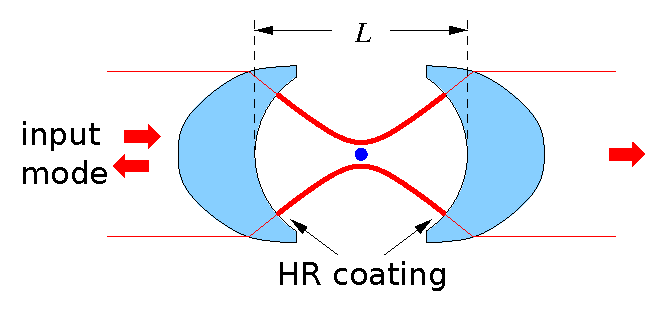
\includegraphics[width=\columnwidth]{cavitything}

            \includegraphics[width=\columnwidth]{coupling_strength.pdf}

        \end{center}
    \end{multicols}

  \figcaption{(Left) The cartoonish picture of our cavity. (Right) The calculated effective mode volume (coming soon). Ignore the current figure on the poster, it is just to bluff those not reading.}

\end{figurehere}

\begin{center}
  {\bf \Large \textsf {Cavity Construction}}
\end{center}

To couple the input mode into the cavity in the near concentric regime, we use anaclastic lens-mirror design, which reduces aberrations and cavity losses of the input mode. We move the mirrors with respect to each other using a 3-dimensional piezo (PZT).

\begin{figurehere}
  \begin{center}
    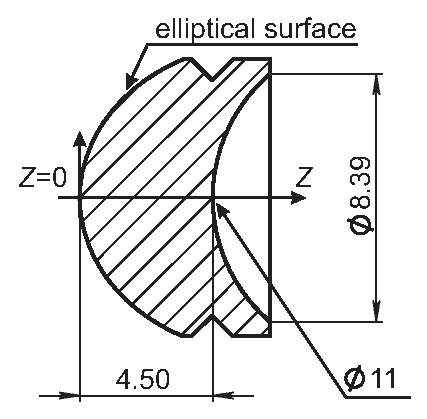
\includegraphics[width=0.3\columnwidth]{cavity_design}
   \hspace*{5cm}
    \includegraphics[width=0.5\columnwidth]{setup_sideon.png}
  \end{center}

  \figcaption{(Left) Anaclastic lens-mirror design. (Right) Anaclastic mirrors are controlled by a 3-axis PZTs for fine alignment.}
\end{figurehere}



\begin{center}
     \begin{center} {\bf \Large \textsf {Experimental Setup}}\end{center}
\end{center}

We stabilise our cavity using off resonant laser (ORL) that is properly referenced to our probe laser. As our cavity has a huge physical volume, we can create a MOT inside the cavity. After the cold atomic cloud from the MOT is formed, a far off resonant laser (FORT), which is the same laser as ORL, will trap single atoms into the cavity mode (kind of random process).

\begin{figurehere}
  \begin{center}
    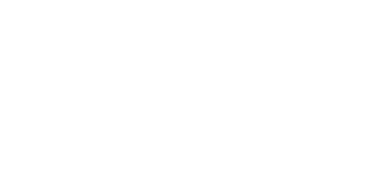
\includegraphics[width=\columnwidth]{stabilise.png}
    \includegraphics[width=\columnwidth]{flou_sig.pdf}
  \end{center}

  \figcaption{(Top) Some figures that is supposed to describe experimental setup. This was the figure that was used in my presentation. Probably need to redraw to incorporate some more things. (Bottom) The fluorescence signal of the MOT scattered by the atom. A quantum jump signal is observed. We now trigger on the occurences of those signal.}
\end{figurehere}

\columnbreak

\begin{center}
     \begin{center} {\bf \Large \textsf {Fluorescence Signal}}\end{center}
\end{center}

We can determined whether we got single atoms or not just by looking at the fluorescence spectrum. If the fluorescence signal drop very sharply, we are confident to claim that it is single atoms. So, after trigger, we send in the fluorescence beam (MOT beam) in and look at the cases. We can confidently determine around 30\% of cases to be single atoms.

\begin{figurehere}
  \begin{center}
    \includegraphics[width=0.4\columnwidth]{Singleatomcases}
   \hspace*{0cm}
    \includegraphics[width=0.4\columnwidth]{Othercases}
  \end{center}

\figcaption{(Left) Samples of the so-called single atom cases. If you don't believe me, see right. (Right) Atom cases that are not single atoms. Depicted are short atom cases (atom that just comes for a very miliseconds to say hi and bye), long atom cases (atoms that want to stick with us probably forever), and multi atom cases.}
\end{figurehere}



\begin{center}
  {\bf \Large \textsf {Transmission Signal}}
\end{center}

We can also monitor the transmission signal as follows. We set the cavity to be resonant with the atom. You can see that right after trigger, the transmission signal is lower, before the atom escapes out of the trap. 

\begin{figurehere}
  \begin{center}
    \includegraphics[width=0.7\columnwidth]{huge_extinction.pdf}
  \end{center}

    \figcaption{You can understand already right? Don't need to explain further right? Hehehehe. In this case, we observed extinction around 30\%}
\end{figurehere}



\begin{center}
  {\bf \Large \textsf {Normal Mode Splitting}}
\end{center}

When we scan the frequency of the laser, we observed a two resolved normal modes, signifying a strong interaction between atom and cavity. We thus estimated the single atom cooperativity to be around 0.4.

\begin{figurehere}
  \begin{center}
    \includegraphics[width=0.7\columnwidth]{triggered_cav_scan.pdf}
  \end{center}

    \figcaption{Baa, baa, black sheep, Have you any wool? Yes, sir, yes, sir, Three bags full;}
\end{figurehere}


\begin{center}
  {\bf \Large \textsf {Outlook}}
\end{center}

Now, we can increase coupling very easy. Just change to new one. After that, we can do all nonsense in quantum information very easily. Hehehehe


\begin{flushleft}
       \begin{center}{\bf \large \textsf {References}}\end{center}
       [1] M.K. Tey et.al., New Journal of Physics {\textbf{11}}, 040311 (2009).
	     \newline
       [2] S.E. Morin, et al., Phys.Rev.Lett., {\textbf {73}} pp.1411 (1994).
       \newline
	     [3] K. Durak et.al., New Journal of Physics {\textbf{16}}, 103002 (2014).

\end{flushleft}
    
\end{multicols}

\end{poster}

\end{document}

